\documentclass[aspectratio=169, table]{beamer}

%\usepackage[beamertheme=./praditatheme]{Pradita}
\usepackage[utf8]{inputenc}
\usepackage{xcolor} % for color
\usepackage{colortbl} % for table color
\usepackage{listings}

% Define Java language style for listings
\lstdefinestyle{JavaStyle}{
language=Java,
basicstyle=\ttfamily\scriptsize,
keywordstyle=\color{blue},
commentstyle=\color{gray},
stringstyle=\color{red},
breaklines=true,
showstringspaces=false,
tabsize=2,
captionpos=b,
numbers=left,
numberstyle=\tiny\color{gray},
frame=lines,
backgroundcolor=\color{lightgray!10},
comment=[l]{//},
morecomment=[s]{/*}{*/},
commentstyle=\color{gray}\ttfamily,
string=[s]{'}{'},
morestring=[s]{"}{"},
%	stringstyle=\color{teal}\ttfamily,
%	showstringspaces=false
}

\usetheme{Pradita}
%
\subtitle{IF220303 - Object-oriented Programming}

\title{\Huge{Structural Patterns 1}\\\vspace{30pt}}
\date[Serial]{\scriptsize {PRU/SPMI/FR-BM-18/0222}}
\author[Pradita]{\small {\textbf{Alfa Yohannis}}}

\begin{document}

\frame{\titlepage}

\begin{frame}[fragile]
\frametitle{Contents}
\vspace{20pt}
\begin{columns}[t]
\column{0.5\textwidth}
\tableofcontents[sections={1-2}]

\column{0.5\textwidth}
\tableofcontents[sections={3-4}]
\end{columns}
\end{frame}


\section{Pola Struktural (Bagian 1)}

\begin{frame}[fragile]{Pola Struktural (Bagian 1): Pengantar}
	\vspace{20pt}
	Pola struktural membantu menyusun kelas dan objek menjadi sistem yang fleksibel dan skalabel.

	\textbf{Fokus utama:}
	\begin{itemize}
		\item Menyederhanakan hubungan antarkomponen.
		\item Memfasilitasi kerja sama antara objek yang berbeda antarmuka.
		\item Mendukung struktur hierarkis dan komposisional.
	\end{itemize}

	\textbf{Pola yang dibahas:}
	\begin{itemize}
		\item \textbf{Adapter} – menjembatani antarmuka yang tidak kompatibel.
		\item \textbf{Decorator} – menambah perilaku tanpa modifikasi kelas asli.
		\item \textbf{Bridge} – memisahkan abstraksi dari implementasi.
		\item \textbf{Composite} – menangani struktur hierarki secara seragam.
	\end{itemize}
\end{frame}


\section{Pola Adapter}

\begin{frame}{\hfill}
	\centering
	\textbf{\Huge{Pola Adapter}}
\end{frame}

\begin{frame}[fragile]{Adapter: Tujuan dan Konteks Penggunaan}
	\vspace{15pt}
	\begin{columns}[T]
		\column{0.55\textwidth}
		\textbf{Tujuan Utama:}
		\begin{itemize}
			\item Menjembatani dua antarmuka yang tidak kompatibel.
			\item Memungkinkan integrasi sistem lama (legacy) atau pustaka eksternal.
			\item Menghindari perubahan pada kode asli (\texttt{Adaptee}).
		\end{itemize}
		
		\textbf{Kapan Digunakan:}
		\begin{itemize}
			\item Kelas eksternal tidak cocok dengan antarmuka sistem kita.
			\item Butuh kompatibilitas tanpa refactor besar.
			\item Klien harus tetap bekerja walau implementasi berubah.
		\end{itemize}
		
		\column{0.45\textwidth}
		\textbf{Cara Kerja:}
		\begin{itemize}
			\item Klien bergantung pada \texttt{Target}.
			\item Adapter mengonversi permintaan ke \texttt{Adaptee}.
			\item \texttt{Adaptee} tetap tidak berubah.
		\end{itemize}
		
		\textbf{Contoh Penerapan:}
		\begin{itemize}
			\item Konversi data XML ke JSON melalui adapter.
			\item Integrasi komponen UI dari framework lama.
			\item USB-to-Serial adapter di perangkat keras.
		\end{itemize}
	\end{columns}
\end{frame}


\begin{frame}[fragile]{Adapter: Contoh Kasus Penggunaan}
	\vspace{20pt}
	\begin{columns}[T]
		\column{0.63\textwidth}
		\textbf{Kasus Umum:}
		\begin{itemize}
			\item Sistem baru butuh JSON, tapi pustaka lama hanya dukung XML.
			\item Komponen \texttt{Swing} ingin dipakai di \texttt{JavaFX}.
			\item Komputer modern terhubung ke perangkat lama via USB-to-Serial.
		\end{itemize}
		
		\textbf{Skenario Nyata:}
		\begin{itemize}
			\item E-commerce integrasi dengan \texttt{PayPal}, \texttt{Stripe}, dan bank lokal.
			\item Gunakan antarmuka tunggal: \texttt{PaymentGateway}.
			\item Adapter menyembunyikan detail API masing-masing.
		\end{itemize}
		
		\column{0.4\textwidth}
		\textbf{Contoh Praktik:}
		\begin{itemize}
			\item Gambar: \texttt{BufferedImage} ke \texttt{Image}.
			\item Android MVVM: Adapter sambung \texttt{View} lama ke \texttt{ViewModel}.
			\item REST API: Adapter ubah request jadi metode mikroservis.
		\end{itemize}
		
		\vspace{8pt}
		\textbf{Manfaat:} Sistem tetap konsisten, fleksibel, dan kompatibel dengan antarmuka lama.
	\end{columns}
\end{frame}


\begin{frame}[fragile]{Adapter: Kelebihan dan Kekurangan}
	\vspace{20pt}
	\begin{columns}[T]
		\column{0.5\textwidth}
		\textbf{Kelebihan:}
		\begin{itemize}
			\item Kompatibel dengan sistem lama tanpa modifikasi.
			\item Mendukung prinsip \textbf{Open/Closed}.
			\item Gunakan kembali kelas lama tanpa refactor.
			\item Menyatukan kelas berbeda di bawah satu antarmuka.
			\item Sederhanakan integrasi dengan pustaka pihak ketiga.
		\end{itemize}
		
		\column{0.5\textwidth}
		\textbf{Kekurangan:}
		\begin{itemize}
			\item Menambah kompleksitas arsitektur.
			\item Berisiko menyembunyikan desain buruk.
			\item Ada sedikit overhead performa.
			\item Terlalu banyak adapter dapat membingungkan.
			\item Tidak cocok untuk perbedaan antarmuka yang besar.
		\end{itemize}
		
		\vspace{10pt}
		\textbf{Catatan:} Gunakan adapter secara selektif untuk menjaga konsistensi dan efisiensi dalam integrasi sistem.
	\end{columns}
\end{frame}

\begin{frame}[fragile]{Struktur UML Pola Adapter}
	\vspace{20pt}
	\begin{figure}
		\centering
		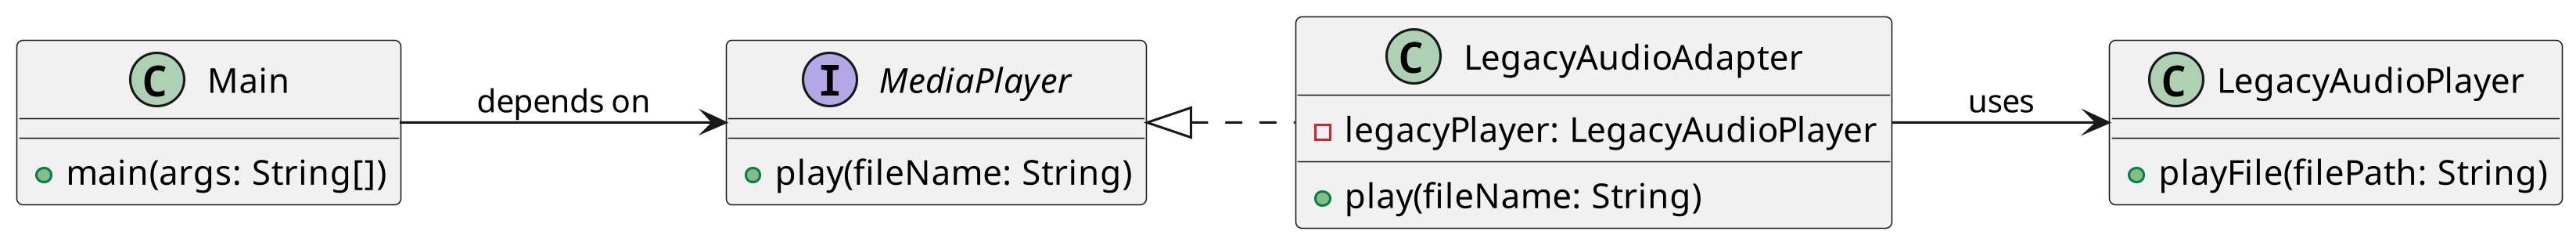
\includegraphics[width=\textwidth]{../../figures/out/adapter.png}
		\caption{Struktur Pola Adapter dengan Komposisi}
	\end{figure}
\end{frame}

\begin{frame}[fragile]{Target Interface: MediaPlayer}
	\vspace{20pt}
	\begin{lstlisting}[style=JavaStyle]
		public interface MediaPlayer {
			void play(String fileName);
		}
	\end{lstlisting}
	\smallskip
	\textit{Antarmuka ini digunakan oleh klien sebagai kontrak standar untuk memutar media.}
\end{frame}

\begin{frame}[fragile]{Adaptee: LegacyAudioPlayer}
	\vspace{20pt}
	\begin{lstlisting}[style=JavaStyle]
		public class LegacyAudioPlayer {
			public void playFile(String filePath) {
				System.out.println("Playing file from legacy player: " + filePath);
			}
		}
	\end{lstlisting}
	\smallskip
	\textit{Kelas lama menyediakan metode yang berbeda (\texttt{playFile}), tidak cocok langsung dengan \texttt{MediaPlayer}.}
\end{frame}

\begin{frame}[fragile]{Adapter: LegacyAudioAdapter}
	\vspace{20pt}
	\begin{lstlisting}[style=JavaStyle]
		public class LegacyAudioAdapter implements MediaPlayer {
			private LegacyAudioPlayer legacyPlayer;
			
			public LegacyAudioAdapter(LegacyAudioPlayer legacyPlayer) {
				this.legacyPlayer = legacyPlayer;
			}
			
			@Override
			public void play(String fileName) {
				legacyPlayer.playFile(fileName);
			}
		}
	\end{lstlisting}
	\smallskip
	\textit{Adapter menjembatani klien dan adaptee dengan menerjemahkan permintaan dari antarmuka \texttt{MediaPlayer}.}
\end{frame}

\begin{frame}[fragile]{Client: Menggunakan Adapter}
	\vspace{20pt}
	\begin{lstlisting}[style=JavaStyle]
		public class Main {
			public static void main(String[] args) {
				MediaPlayer player =
				new LegacyAudioAdapter(new LegacyAudioPlayer());
				player.play("music.mp3");
			}
		}
	\end{lstlisting}
	\smallskip
	\textit{Klien menggunakan antarmuka \texttt{MediaPlayer} tanpa mengetahui bahwa implementasinya membungkus kelas lama.}
\end{frame}


\section{Pola Decorator}

\begin{frame}{\hfill}
	\centering
	\textbf{\Huge{Pola Decorator}}
\end{frame}

\begin{frame}[fragile]{Decorator: Tujuan dan Konteks Penggunaan}
	\vspace{20pt}
	\begin{columns}[t]
		\column{0.5\textwidth}
		\textbf{Deskripsi Umum:}
		
		Pola \textit{Decorator} menambahkan tanggung jawab baru secara dinamis ke objek tanpa mengubah kelas dasarnya, dengan membungkus objek dalam kelas lain (\texttt{Decorator}) yang memakai antarmuka yang sama.
		
		\vspace{6pt}
		\textbf{Prinsip Desain:}
		\begin{itemize}
			\item \textbf{Open/Closed Principle}
			\item \textbf{Single Responsibility Principle}
		\end{itemize}
		
		\column{0.5\textwidth}
		\textbf{Kapan Digunakan:}
		\begin{itemize}
			\item Menambah fitur ke objek tertentu saja.
			\item Menghindari pewarisan kompleks.
			\item Perilaku tambahan perlu disusun berlapis.
		\end{itemize}
		
		\vspace{4pt}
		\textbf{Contoh Praktis:}
		\begin{itemize}
			\item GUI: Tombol dengan border, shadow, tooltip.
			\item Java I/O: \texttt{BufferedReader}, \texttt{InputStreamReader}.
		\end{itemize}
	\end{columns}
\vspace{5pt}
	Pendekatan ini menghasilkan sistem yang modular, fleksibel, dan mudah diperluas tanpa memperumit pewarisan.
\end{frame}



\begin{frame}[fragile]{Decorator: Contoh Kasus Penggunaan}
	\vspace{15pt}
	\begin{columns}[T]
		\column{0.5\textwidth}
		Pola \textit{Decorator} ideal untuk menambahkan perilaku baru ke objek tertentu tanpa memengaruhi kelas lainnya. Cocok untuk sistem yang membutuhkan fleksibilitas tinggi.
		
		\vspace{10pt}
		\textbf{Contoh nyata:}
		\begin{itemize}
			\item \textbf{UI:} \texttt{TextField} dengan \texttt{BorderDecorator}, \texttt{ScrollDecorator}, \texttt{TooltipDecorator}.
			\item \textbf{Java I/O:} \texttt{InputStream} dibungkus \texttt{BufferedInputStream}, \texttt{DataInputStream}.
		\end{itemize}
		
		\column{0.5\textwidth}
		\begin{itemize}
			\item \textbf{Notifikasi:} \texttt{Notifier} dihias dengan \texttt{EmailNotifier}, \texttt{SMSNotifier}.
			\item \textbf{Game:} \texttt{Player} dengan \texttt{ShieldDecorator}, \texttt{SpeedBoostDecorator}.
		\end{itemize}
		
		\vspace{5pt}
		\textbf{Contoh kode:}
\begin{lstlisting}[style=JavaStyle]
InputStream input = new BufferedInputStream(
new FileInputStream("data.txt"));
\end{lstlisting}
			\vspace{5pt}
		Decorator memberikan fleksibilitas tinggi tanpa menciptakan banyak subclass yang kompleks.
	\end{columns}
	

\end{frame}


\begin{frame}[fragile]{Decorator: Kelebihan dan Kekurangan}
	\vspace{20pt}
	\begin{columns}[T]
		\column{0.5\textwidth}
		\textbf{Kelebihan:}
		\begin{itemize}
			\item Tambah fitur tanpa ubah kelas asli.
			\item Gunakan komposisi, bukan pewarisan.
			\item Mendukung prinsip \textit{Open/Closed}.
			\item Setiap decorator punya satu tanggung jawab.
			\item Kombinasi decorator fleksibel dan modular.
		\end{itemize}
		
		\column{0.5\textwidth}
		\textbf{Kekurangan:}
		\begin{itemize}
			\item Struktur bisa kompleks dan sulit ditelusuri.
			\item Debugging lebih sulit karena logika tersebar.
			\item Jumlah kelas meningkat seiring banyak fitur.
			\item Bergantung pada konsistensi antarmuka.
			\item Potensi over-engineering untuk kasus sederhana.
		\end{itemize}
	\end{columns}
	
	\vspace{5pt}
	Gunakan secara selektif saat perluas perilaku objek tanpa memperbesar hirarki pewarisan.
\end{frame}


\begin{frame}[fragile]{Decorator Pattern: Struktur UML}
	\vspace{20pt}
	\begin{figure}[h]
		\centering
		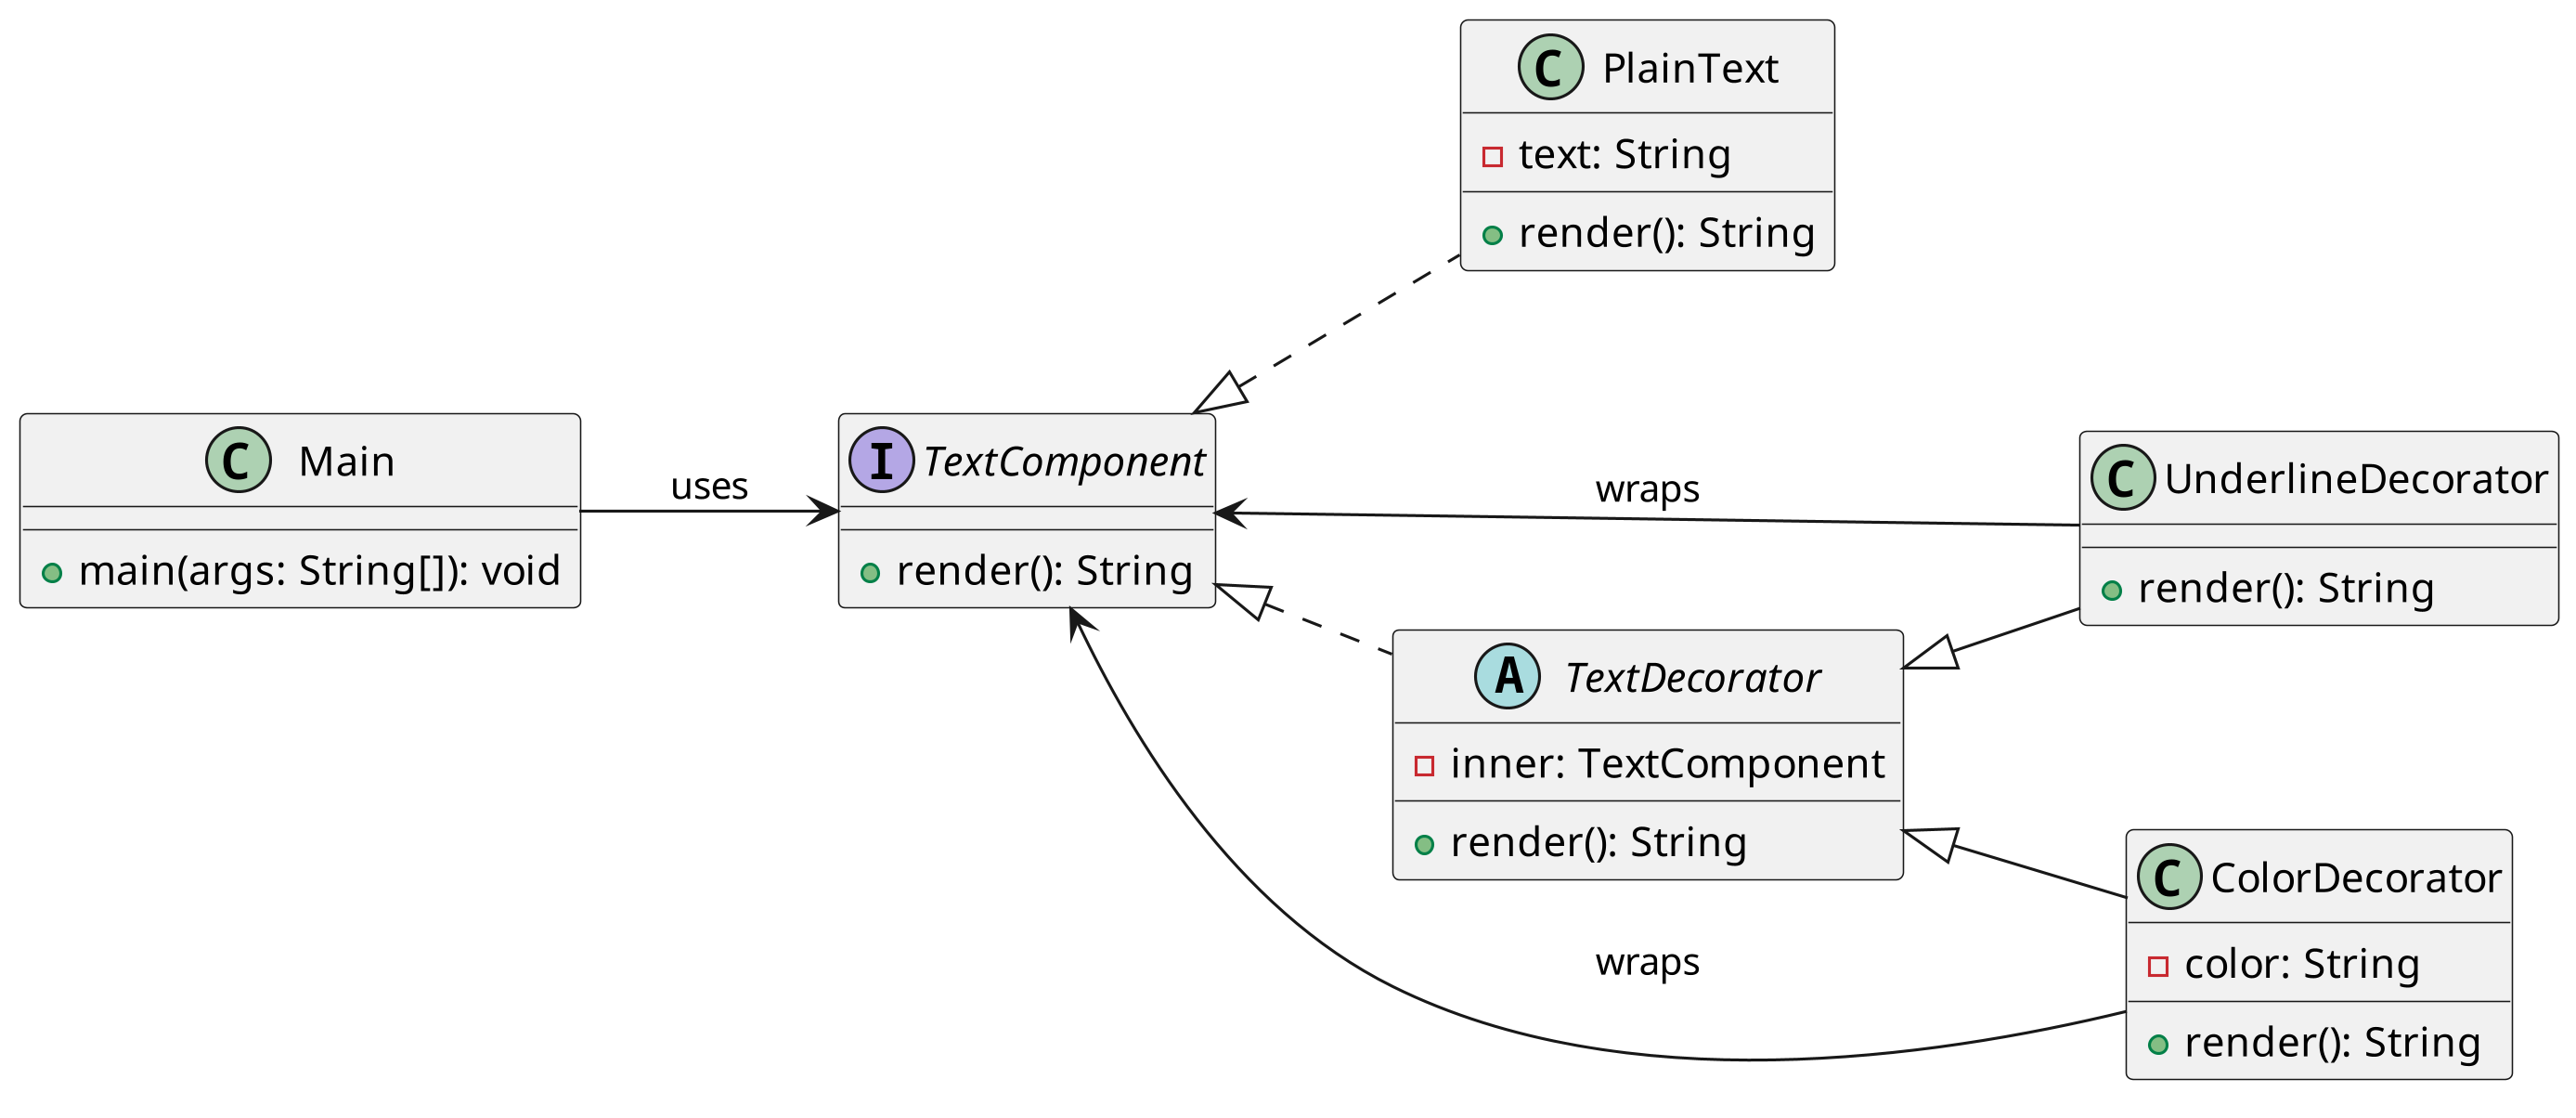
\includegraphics[width=\textwidth]{../../figures/out/decorator.png}
		\label{fig:decorator}
	\end{figure}
\end{frame}

\begin{frame}[fragile]{Komponen Dasar: TextComponent}
	\vspace{20pt}
	\begin{lstlisting}[style=JavaStyle]
		public interface TextComponent {
			String render();
		}
	\end{lstlisting}
	\small
	Antarmuka dasar yang akan digunakan oleh komponen konkret maupun decorator. Semua objek dekorasi akan mengikuti kontrak ini.
\end{frame}

\begin{frame}[fragile]{Komponen Konkret: PlainText}
	\vspace{20pt}
	\begin{lstlisting}[style=JavaStyle]
		public class PlainText implements TextComponent {
			private String text;
			
			public PlainText(String text) {
				this.text = text;
			}
			
			@Override
			public String render() {
				return text;
			}
		}
	\end{lstlisting}
	\small
	Kelas \texttt{PlainText} adalah implementasi konkret dari \texttt{TextComponent} yang menyimpan dan mengembalikan teks biasa.
\end{frame}

\begin{frame}[fragile]{Decorator Abstrak: TextDecorator}
	\vspace{20pt}
	\begin{lstlisting}[style=JavaStyle]
		public abstract class TextDecorator implements TextComponent {
			protected TextComponent inner;
			
			public TextDecorator(TextComponent inner) {
				this.inner = inner;
			}
			
			public abstract String render();
		}
	\end{lstlisting}
	\small
	Kelas abstrak \texttt{TextDecorator} menyimpan referensi ke objek \texttt{TextComponent} lain dan mewariskan metode \texttt{render()}.
\end{frame}

\begin{frame}[fragile]{Decorator Konkret: UnderlineDecorator}
	\vspace{20pt}
	\begin{lstlisting}[style=JavaStyle]
		public class UnderlineDecorator extends TextDecorator {
			public UnderlineDecorator(TextComponent inner) {
				super(inner);
			}
			
			@Override
			public String render() {
				return "<u>" + inner.render() + "</u>";
			}
		}
	\end{lstlisting}
	\small
	\texttt{UnderlineDecorator} menambahkan tag HTML \texttt{<u>} untuk membuat teks bergaris bawah.
\end{frame}

\begin{frame}[fragile]{Decorator Konkret: ColorDecorator}
	\vspace{20pt}
	\begin{lstlisting}[style=JavaStyle]
		public class ColorDecorator extends TextDecorator {
			private String color;
			
			public ColorDecorator(TextComponent inner, String color) {
				super(inner);
				this.color = color;
			}
			
			@Override
			public String render() {
				return "<span style='color:" + color + "'>" +
				inner.render() + "</span>";
			}
		}
	\end{lstlisting}
	\small
	\texttt{ColorDecorator} membungkus teks dengan warna tertentu menggunakan tag \texttt{<span>}.
\end{frame}

\begin{frame}[fragile]{Client: Penggunaan Decorator}
	\vspace{20pt}
	\begin{lstlisting}[style=JavaStyle]
		public class Main {
			public static void main(String[] args) {
				TextComponent text = new PlainText("Hello, Decorator!");
				TextComponent decorated = new ColorDecorator(
				new UnderlineDecorator(text), "blue");
				
				System.out.println(decorated.render());
			}
		}
	\end{lstlisting}
	\small
	Client menghias \texttt{PlainText} dengan garis bawah dan warna biru menggunakan dua decorator secara bertingkat.
\end{frame}

\begin{frame}[fragile]{Hasil Output dan Kesimpulan}
	\vspace{20pt}
	\begin{verbatim}
		<span style='color:blue'><u>Hello, Decorator!</u></span>
	\end{verbatim}
	\small
	Output menunjukkan kombinasi dekorasi yang modular. Dengan pendekatan ini, kita dapat menambah atau menggabungkan fitur secara dinamis tanpa mengubah kelas dasar.
\end{frame}

\section{Pola Bridge}

\begin{frame}{\hfill}
	\centering
	\textbf{\Huge{Pola Bridge}}
\end{frame}

\begin{frame}[fragile]{Bridge: Tujuan dan Konteks Penggunaan}
	\vspace{20pt}
	\begin{columns}[T]
		\column{0.55\textwidth}
		\textbf{Tujuan Pola Bridge:}
		\begin{itemize}
			\item Memisahkan abstraksi dari implementasi agar keduanya bisa berkembang independen.
			\item Menghindari hierarki pewarisan yang kompleks dan tidak scalable.
			\item Menyediakan struktur fleksibel untuk dua dimensi variasi.
		\end{itemize}
		
		\textbf{Struktur:}
		\begin{enumerate}
			\item \textbf{Abstraction:} Antarmuka/kelas utama yang digunakan klien dan menyimpan referensi ke \texttt{Implementor}.
			\item \textbf{Implementor:} Antarmuka untuk detail teknis yang bisa diubah mandiri.
		\end{enumerate}
		
		\column{0.45\textwidth}
		\textbf{Kapan Digunakan:}
		\begin{itemize}
			\item Terdapat dua dimensi variasi (misal: bentuk \& platform).
			\item Sistem perlu fleksibilitas dan modularitas tinggi.
			\item Menghindari ledakan kombinasi subclass akibat pewarisan ganda.
		\end{itemize}
		
		\textbf{Contoh Umum:}
		\begin{itemize}
			\item Rendering bentuk di OpenGL vs HTML Canvas.
			\item Format dokumen (PDF, DOCX) vs metode penyimpanan.
			\item Aplikasi UI lintas sistem operasi.
		\end{itemize}
	\end{columns}
\end{frame}

\begin{frame}[fragile]{Bridge Pattern: Contoh Kasus Penggunaan}
	\vspace{20pt}
	\begin{columns}[T]
		\column{0.55\textwidth}
		\textbf{Masalah:} Dua dimensi variasi → \textbf{ledakan subclass}.
		
		\textbf{Contoh 1:} Gambar Bentuk
		\begin{itemize}
			\item Bentuk: \texttt{Circle}, \texttt{Rectangle}, \texttt{Triangle}
			\item Renderer: OpenGL, DirectX, Canvas
			\item Tanpa Bridge: \texttt{CircleWithOpenGL}, dst.
			\item Dengan Bridge: Bentuk dan renderer dipisah via komposisi.
		\end{itemize}
		
		\textbf{Contoh 2:} UI Lintas Platform
		\begin{itemize}
			\item Abstraksi: \texttt{Window}, \texttt{Dialog}, \texttt{Button}
			\item Platform: \texttt{WinAPI}, \texttt{GTK}, \texttt{Qt}
		\end{itemize}
		
		\column{0.45\textwidth}
		\textbf{Contoh 3:} Simpan Dokumen
		\begin{itemize}
			\item Jenis: \texttt{Invoice}, \texttt{Report}, \texttt{Letter}
			\item Storage: \texttt{FileSystem}, \texttt{Database}, \texttt{Cloud}
			\item Bridge → fleksibel pilih penyimpanan tanpa subclass.
		\end{itemize}
		
		\vspace{4pt}
		\textbf{Kesimpulan:} Bridge pisahkan variasi dan gabungkan fleksibel saat runtime.
	\end{columns}
\end{frame}



\begin{frame}[fragile]{Bridge Pattern: Kelebihan dan Kekurangan}
	\vspace{20pt}
	\begin{columns}[T]
		\column{0.48\textwidth}
		\textbf{Kelebihan:}
		\begin{itemize}
			\item Memisahkan abstraksi dari implementasi.
			\item Mendukung perluasan multidimensi tanpa ledakan subclass.
			\item Sejalan dengan prinsip Open/Closed dan SRP.
			\item Modular dan mudah diuji per hierarki.
			\item Adaptif terhadap teknologi baru (renderer, platform, protokol).
		\end{itemize}
		
		\column{0.48\textwidth}
		\textbf{Kekurangan:}
		\begin{itemize}
			\item Struktur kode lebih kompleks dibanding pewarisan langsung.
			\item Butuh pemahaman desain yang lebih matang.
			\item Tidak efisien untuk sistem sederhana (overengineering).
			\item Pemeliharaan dua hierarki terpisah.
			\item Rawan pelanggaran pemisahan tanggung jawab jika rancangan lemah.
		\end{itemize}
	\end{columns}
\end{frame}


\begin{frame}[fragile]{Bridge Pattern: Struktur UML}
	\vspace{20pt}
	Struktur UML menunjukkan pemisahan antara abstraksi dan implementasi melalui komposisi. 
	Hal ini memungkinkan perluasan fleksibel tanpa modifikasi kelas yang ada.
	
	\begin{figure}
		\centering
		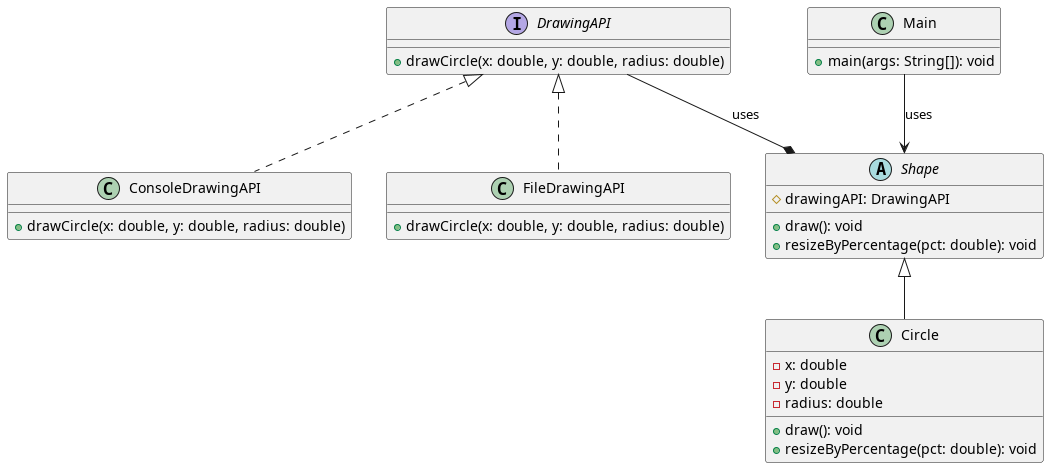
\includegraphics[width=0.9\textwidth]{../../figures/out/bridge.png}
		\label{fig:bridge}
	\end{figure}
\end{frame}

\begin{frame}[fragile]{Bridge Pattern: Interface Implementor}
	\vspace{20pt}
	Antarmuka \texttt{DrawingAPI} mendefinisikan operasi dasar yang harus diimplementasikan oleh setiap renderer. 
	Bridge mengandalkan antarmuka ini untuk menyambungkan ke detail implementasi.
	
	\begin{lstlisting}[style=JavaStyle]
		public interface DrawingAPI {
			void drawCircle(double x, double y, double radius);
		}
	\end{lstlisting}
\end{frame}

\begin{frame}[fragile]{Bridge Pattern: Implementasi Renderer}
\vspace{20pt}
Dua implementasi \texttt{DrawingAPI} menggambarkan variasi renderer—satu menampilkan ke konsol, lainnya menulis ke file. 
Mereka mengimplementasikan metode yang sama namun dengan perilaku berbeda.

\begin{lstlisting}[style=JavaStyle]
public class ConsoleDrawingAPI implements DrawingAPI {
	@Override
	public void drawCircle(double x, double y, double radius) {
		System.out.println("Console: Drawing circle at (" + x + "," + y + ") with radius " + radius);
	}
}

public class FileDrawingAPI implements DrawingAPI {
	@Override
	public void drawCircle(double x, double y, double radius) {
		System.out.println("File: Writing 'Circle (" + x + "," + y + ") radius " + radius + "' to file.");
	}
}
\end{lstlisting}
\end{frame}

\begin{frame}[fragile]{Bridge Pattern: Abstraksi}
	\vspace{20pt}
	\texttt{Shape} adalah kelas abstrak yang mendefinisikan struktur bentuk dan menyimpan referensi ke renderer. 
	Abstraksi ini tidak tahu detail teknis dari proses rendering.
	
	\begin{lstlisting}[style=JavaStyle]
		public abstract class Shape {
			protected DrawingAPI drawingAPI;
			
			protected Shape(DrawingAPI drawingAPI) {
				this.drawingAPI = drawingAPI;
			}
			
			public abstract void draw();
			public abstract void resizeByPercentage(double pct);
		}
	\end{lstlisting}
\end{frame}

\begin{frame}[fragile]{Bridge: Circle sebagai Abstraksi Konkret}
\vspace{20pt}
\texttt{Circle} adalah bentuk konkret yang merealisasikan abstraksi dan mendelegasikan operasinya ke \texttt{DrawingAPI}. Ia tidak peduli renderer mana yang digunakan selama mengikuti kontrak.

\begin{columns}[T]
\column{0.5\textwidth}
\begin{lstlisting}[style=JavaStyle, basicstyle=\ttfamily\scriptsize]
public class Circle extends Shape {
	private double x, y, radius;
	
	public Circle(double x, double y, double radius,
	DrawingAPI drawingAPI) {
		super(drawingAPI);
		this.x = x;
		this.y = y;
		this.radius = radius;
	}
\end{lstlisting}

\column{0.5\textwidth}
\begin{lstlisting}[style=JavaStyle, basicstyle=\ttfamily\scriptsize]
	@Override
	public void draw() {
		drawingAPI.drawCircle(x, y, radius);
	}
	
	@Override
	public void resizeByPercentage(double pct) {
		radius *= (1.0 + pct / 100.0);
	}
}
\end{lstlisting}
\end{columns}
\end{frame}


\begin{frame}[fragile]{Bridge Pattern: Client}
	\vspace{20pt}
	Klien menggunakan abstraksi \texttt{Shape} dan menyuntikkan implementasi \texttt{DrawingAPI} saat instansiasi. 
	Bridge memisahkan logika bentuk dari detail teknik gambar.
	
\begin{lstlisting}[style=JavaStyle]
	public class Main {
		public static void main(String[] args) {
			Shape circle1 = new Circle(1, 2, 3, new ConsoleDrawingAPI());
			Shape circle2 = new Circle(5, 7, 10, new FileDrawingAPI());
			
			circle1.draw(); // Output ke konsol
			circle2.draw(); // Simulasi output ke file
		}
	}
\end{lstlisting}
\end{frame}

\begin{frame}[fragile]{Bridge Pattern: Ringkasan Implementasi}
	\vspace{20pt}
	Pola Bridge memisahkan hierarki bentuk dari renderer untuk menghindari ledakan subclass. 
	Abstraksi dan implementasi berkembang mandiri tanpa saling memengaruhi.
	
	\begin{itemize}
		\item \texttt{DrawingAPI}: mendefinisikan metode rendering bentuk.
		\item \texttt{ConsoleDrawingAPI} dan \texttt{FileDrawingAPI}: implementasi teknik rendering.
		\item \texttt{Shape}: abstraksi yang menyimpan referensi ke \texttt{DrawingAPI}.
		\item \texttt{Circle}: bentuk konkret yang menggunakan renderer sesuai kebutuhan.
	\end{itemize}
\end{frame}

\section{Pola Composite}

\begin{frame}{\hfill}
	\centering
	\textbf{\Huge{Pola Composite}}
\end{frame}

\begin{frame}[fragile]{Composite: Tujuan dan Konteks Penggunaan}
	\vspace{20pt}
	Pola \textit{Composite} memungkinkan objek tunggal dan kumpulan objek diperlakukan secara seragam dalam struktur hierarkis seperti pohon.

	\begin{columns}[T]
		\column{0.6\textwidth}
		\textbf{Tujuan utama:}
		\begin{itemize}
			\item Satukan objek sederhana dan kompleks dalam satu struktur.
			\item Izinkan operasi rekursif pada struktur hierarki.
			\item Sederhanakan logika klien dengan antarmuka seragam.
		\end{itemize}
		
		\textbf{Struktur pola:}
		\begin{enumerate}
			\item \texttt{Component}: antarmuka umum.
			\item \texttt{Leaf}: objek individu.
			\item \texttt{Composite}: objek yang berisi anak-anak.
		\end{enumerate}
		
		\column{0.4\textwidth}
		\textbf{Kapan digunakan:}
		\begin{itemize}
			\item Saat data disusun dalam bentuk pohon.
			\item Saat operasi perlu dipanggil secara seragam.
			\item Saat struktur data bersifat dinamis dan bersarang.
		\end{itemize}
		
		\textbf{Contoh nyata:} Struktur file dan folder, Panel dan elemen UI, Dokumen HTML/XML bersarang.
	\end{columns}
\end{frame}

\begin{frame}[fragile]{Composite: Contoh Kasus Penggunaan}
	\vspace{20pt}
	Pola \textit{Composite} menyatukan objek individual dan komposit dalam satu antarmuka agar dapat diproses secara seragam.
	
	\begin{columns}[T]
		\column{0.45\textwidth}
		\textbf{Contoh Umum:}
		\begin{itemize}
			\item \textbf{File System:} \texttt{File} dan \texttt{Directory} implementasikan antarmuka \texttt{FileSystemNode}.
			\item \textbf{Antarmuka GUI:} \texttt{Panel}, \texttt{Button}, \texttt{TextField} diolah melalui \texttt{UIComponent}.
			\item \textbf{Struktur Organisasi:} \texttt{Employee}, \texttt{Team}, \texttt{Department} mengimplementasikan \texttt{OrganizationUnit}.
		\end{itemize}
		
		\column{0.55\textwidth}
		\textbf{Contoh Praktik Lain:}
		\begin{itemize}
			\item Struktur tugas dan sub-tugas dalam manajemen proyek.
			\item Hierarki menu aplikasi desktop atau web.
			\item Perakitan produk dengan sub-komponen dalam kalkulasi biaya produksi.
		\end{itemize}
		
		\vspace{5pt}
		Semua entitas diproses secara rekursif, memungkinkan kode yang konsisten, modular, dan mudah dikembangkan.
	\end{columns}
\end{frame}


\begin{frame}[fragile]{Composite: Kelebihan dan Kekurangan}
	\vspace{15pt}
	Pola \textit{Composite} cocok untuk struktur hierarki dan memungkinkan pemrosesan objek leaf dan composite secara seragam.
	
	\begin{columns}[T]
		\column{0.47\textwidth}
		\textbf{Kelebihan:}
		\begin{itemize}
			\item Menyederhanakan logika klien karena antarmuka seragam.
			\item Cocok untuk struktur rekursif seperti file system.
			\item Mendukung prinsip Open/Closed untuk perluasan.
			\item Modular dan dapat digunakan ulang.
			\item Mendukung agregasi data secara rekursif.
		\end{itemize}
		
		\column{0.53\textwidth}
		\textbf{Kekurangan:}
		\begin{itemize}
			\item Sulit membatasi penambahan anak pada leaf.
			\item Overhead tidak diperlukan untuk struktur sederhana.
			\item Menyembunyikan perbedaan antara leaf dan composite.
			\item Debugging struktur dalam menjadi kompleks.
			\item Manajemen dependensi dan konsistensi lebih sulit.
		\end{itemize}
	\end{columns}
\end{frame}

\begin{frame}[fragile]{Struktur Pola Composite}
	\vspace{20pt}
	Struktur pola \textit{Composite} membedakan antara leaf dan composite, namun keduanya mengikuti antarmuka yang sama.
	
	\begin{figure}[h]
		\centering
		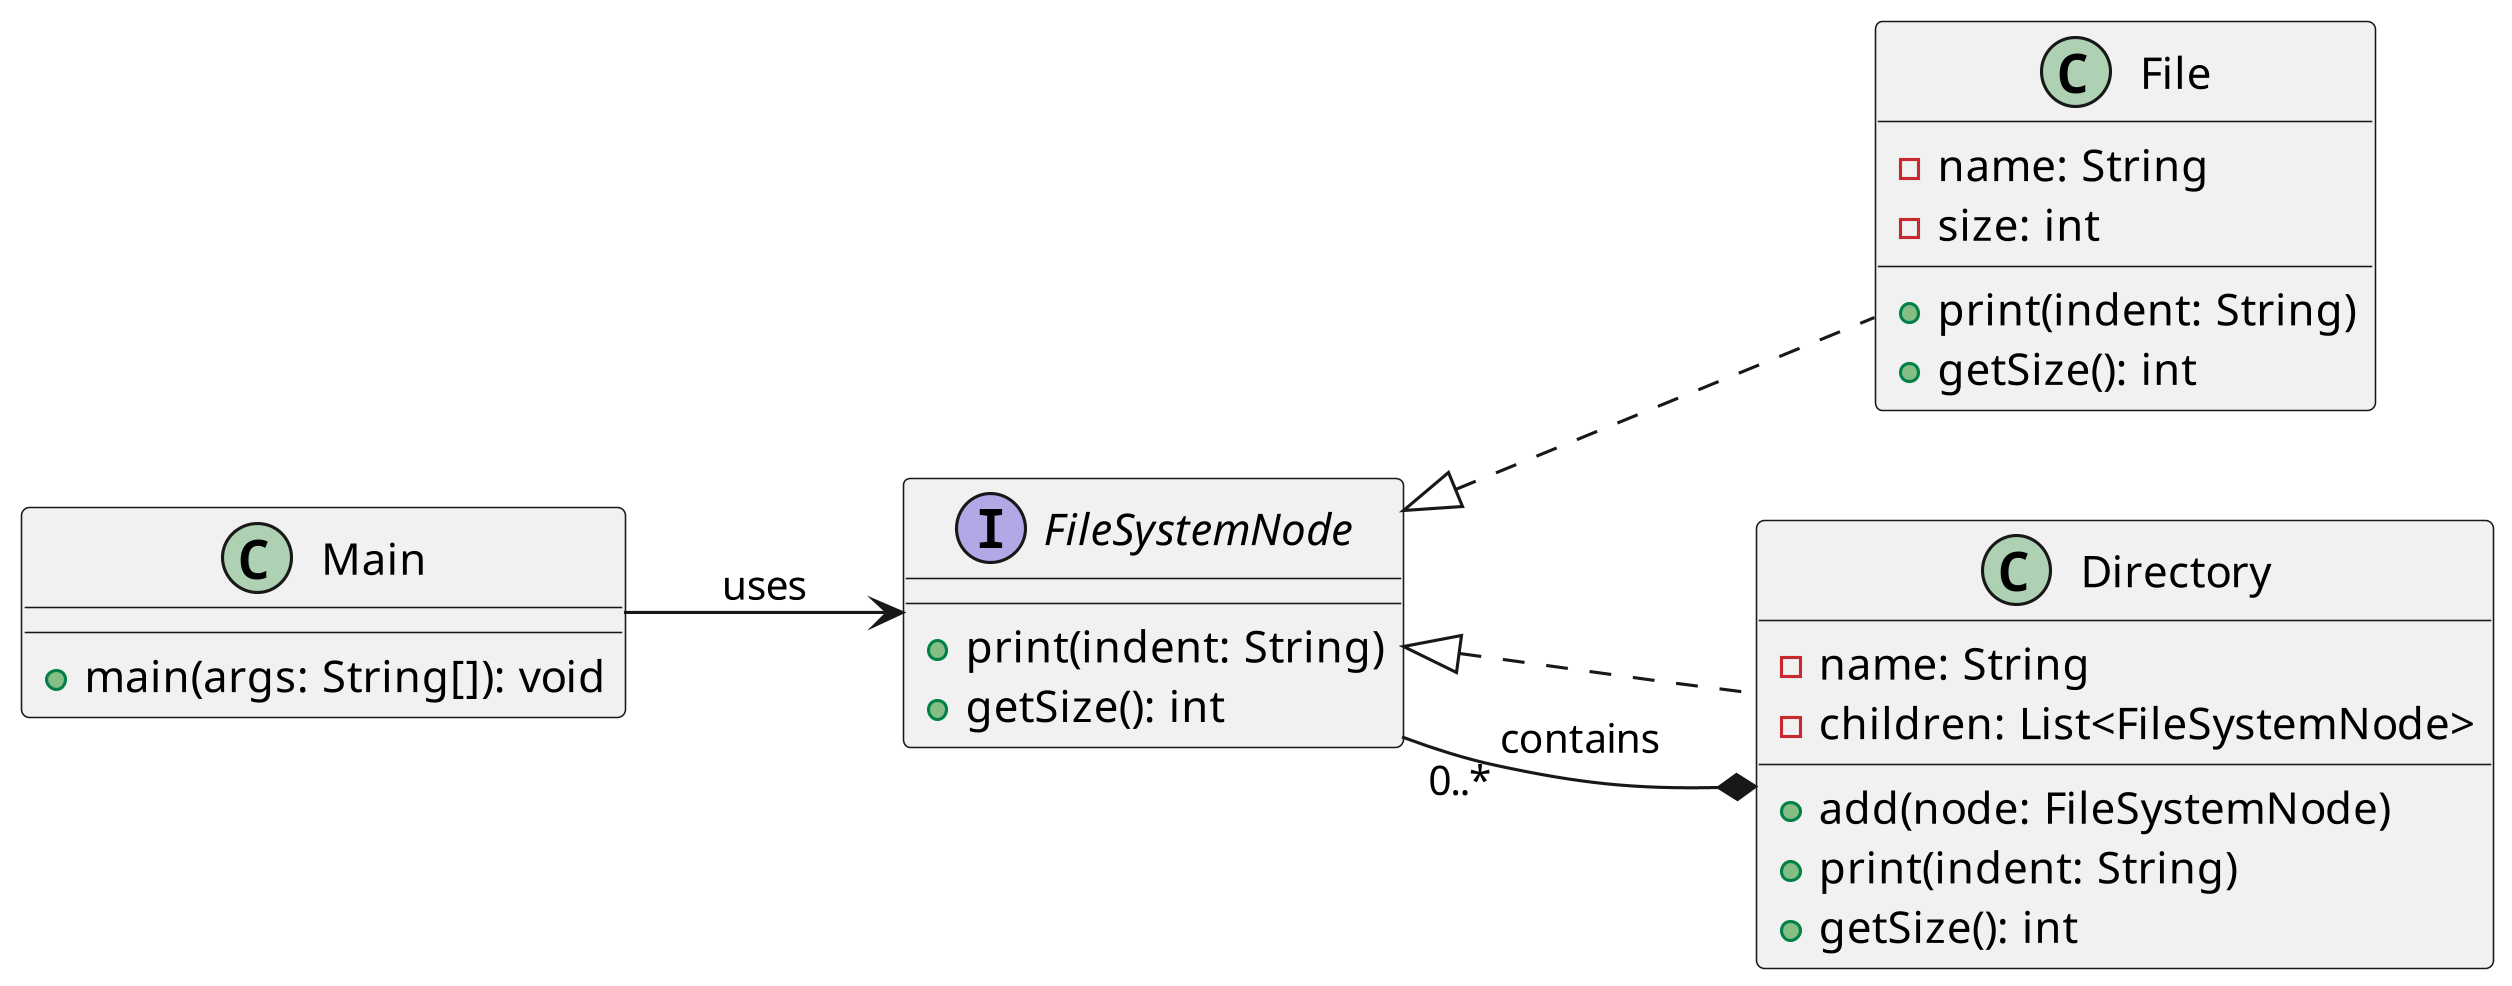
\includegraphics[width=\textwidth]{../../figures/out/composite.png}
	\end{figure}
\end{frame}

\begin{frame}[fragile]{Component dan Leaf}
\vspace{20pt}
\texttt{FileSystemNode} adalah antarmuka dasar. \texttt{File} mewakili objek leaf yang tidak memiliki anak.

\begin{columns}[T]
\column{0.5\textwidth}
\begin{lstlisting}[style=JavaStyle, basicstyle=\ttfamily\scriptsize]
public interface FileSystemNode {
	void print(String indent);
	int getSize();
}

public class File implements FileSystemNode {
	private String name;
	private int size;
	
	public File(String name, int size) {
		this.name = name;
		this.size = size;
	}
\end{lstlisting}

\column{0.5\textwidth}
\begin{lstlisting}[style=JavaStyle, basicstyle=\ttfamily\scriptsize]
	@Override
	public void print(String indent) {
		System.out.println(indent + "- File: " + name + " (" + size + "KB)");
	}
	
	@Override
	public int getSize() {
		return size;
	}
}
\end{lstlisting}
\end{columns}
\end{frame}


\begin{frame}[fragile]{Composite: Directory}
\vspace{20pt}
Kelas \texttt{Directory} mewakili composite yang menyimpan daftar \texttt{FileSystemNode} lain secara rekursif.

\begin{columns}[T]
\column{0.5\textwidth}
\begin{lstlisting}[style=JavaStyle, basicstyle=\ttfamily\scriptsize]
import java.util.ArrayList;
import java.util.List;

public class Directory implements FileSystemNode {
	private String name;
	private List<FileSystemNode> 
	children = new ArrayList<>();
	
	public Directory(String name) {
		this.name = name;
	}
	
	public void add(FileSystemNode node) {
		children.add(node);
	}
\end{lstlisting}

\column{0.5\textwidth}
\begin{lstlisting}[style=JavaStyle, basicstyle=\ttfamily\scriptsize]
	@Override
	public void print(String indent) {
		System.out.println(indent + "+ Directory: " + name);
		for (FileSystemNode child : children) {
			child.print(indent + "  ");
		}
	}
	@Override
	public int getSize() {
		int totalSize = 0;
		for (FileSystemNode child : children) {
			totalSize += child.getSize();
		}
		return totalSize;
	}
}
\end{lstlisting}
\end{columns}
\end{frame}


\begin{frame}[fragile]{Client: Membentuk Struktur File}
	\vspace{20pt}
	Klien membuat struktur folder dan file, lalu mencetak isi dan total ukurannya secara rekursif.
	
	\begin{lstlisting}[style=JavaStyle]
		public class Main {
			public static void main(String[] args) {
				File file1 = new File("resume.pdf", 120);
				File file2 = new File("budget.xlsx", 200);
				File file3 = new File("notes.txt", 30);
				Directory docs = new Directory("Documents");
				docs.add(file1);
				docs.add(file2);
				
				Directory root = new Directory("Home");
				root.add(docs);
				root.add(file3);
				root.print(""); // Cetak struktur
				System.out.println("Total size: " + root.getSize() + "KB");
			}
		}
	\end{lstlisting}
\end{frame}

\begin{frame}[fragile]{Penjelasan}
	\vspace{20pt}
	Semua node memiliki antarmuka yang sama sehingga dapat diproses secara seragam tanpa logika kondisional tambahan.
	
	\begin{itemize}
		\item \texttt{FileSystemNode} menyatukan \texttt{Leaf} dan \texttt{Composite} dalam satu kontrak.
		\item Struktur pohon dapat berkembang secara fleksibel dan rekursif.
		\item Operasi seperti \texttt{print()} dan \texttt{getSize()} cukup dipanggil satu kali di root.
		\item Klien tidak perlu mengetahui apakah node adalah file atau direktori.
	\end{itemize}
\end{frame}

\begin{frame}[fragile]{Kesimpulan}
	\vspace{20pt}
	Pola-pola struktural seperti \textit{Adapter}, \textit{Decorator}, \textit{Bridge}, dan \textit{Composite} menawarkan solusi elegan untuk mengelola relasi antar kelas dan objek dalam perangkat lunak.
	
	\vspace{10pt}
	\begin{itemize}
		\item \textbf{Adapter:} Menghubungkan kelas dengan antarmuka berbeda.
		\item \textbf{Decorator:} Menambahkan fitur ke objek tanpa mengubah kelas aslinya.
		\item \textbf{Bridge:} Memisahkan abstraksi dari implementasi agar dapat berkembang terpisah.
		\item \textbf{Composite:} Memperlakukan objek tunggal dan grup secara seragam.
	\end{itemize}
	
	\vspace{10pt}
	Penerapan pola yang tepat membantu membangun sistem yang modular, fleksibel, dan mudah dirawat. Pilih pola sesuai kebutuhan agar desain tetap bersih dan scalable.
\end{frame}



\end{document}
                                                                                                                                                                               